\documentclass[compress,xcolor=table]{beamer}
% add handout to optional args for handout version

\usepackage{beamerthemesplit}
\usepackage[utf8]{inputenc}
\usepackage[german]{babel}
\usepackage{german}
\usepackage{graphicx}
\usepackage{subfigure}
\usepackage{epsfig}
\usepackage{tabularx}
\usepackage{latexsym}
\usepackage{url}
\usepackage{tikz}
\usepackage{multimedia}
\usepackage{xcolor}
\usepackage{eso-pic}
\usepackage{color}
\usepackage{type1cm}
\usepackage{listings}
\usepackage{verbatim}
\usepackage{colortbl}
\usepackage{psfrag}
\usepackage{xifthen}
\usepackage[absolute,overlay]{textpos}
\usepackage{palatino}
\usepackage{appendixnumberbeamer}

%% Mulberry Color for highlighting
\definecolor{Mulberry}{cmyk}{0.34,0.90,0,0.02}
\definecolor{Lavender}{cmyk}{0,0.48,0,0}
\definecolor{Melon}{cmyk}{0,0.46,0.50,0}
\definecolor{Peach}{cmyk}{0,0.50,0.70,0}
\definecolor{RedOrange}{cmyk}{0,0.77,0.87,0}
\definecolor{BrickRed}{cmyk}{0,0.89,0.94,0.28}
\definecolor{Mahogany}{cmyk}{0,0.85,0.87,0.35}
\definecolor{BurntOrange}{cmyk}{0,0.51,1,0}
\definecolor{BitterSweet}{cmyk}{0,0.75,1,0.24}
\definecolor{FawkesRed}{rgb}{0.53,0,0}
\definecolor{RosBlue}{rgb}{0.19,0.25,0.38}


\mode<presentation>
{
  \usetheme{FawkesSimple}

  % to hide nav bar uncomment this line
  \setbeamertemplate{navigation symbols}{}

  %\setbeamercovered{transparent}
  \setbeamercovered{%
    again covered={\opaqueness<1->{40}}
  }
}

% Usage notes for handout version:
% Compile the beamer version immediately before you build the handout version,
% otherwise page numbers etc. will be wrong! The .aux files are *not* updated
% in handout mode, see PGF Manual for details why this is necessary.
% Comment out below one of the two pgfuselayout lines for either 2 or 4 slides
% per page. To have a very light grey background uncomment the background canvas
% color line. The logical page options are used to draw borders around each
% slide.
\mode<handout>
{
  \usetheme{Fawkes}

  % to hide nav bar uncomment this line
  \setbeamertemplate{navigation symbols}{}

  %\setbeamercovered{transparent}
  \setbeamercovered{%
    again covered={\opaqueness<1->{40}}
  }

  % Very slight grey background, can be used instead of borders
  %\setbeamercolor{background canvas}{bg=black!5}

  \usepackage{pgfpages}
  \pgfpagesuselayout{4 on 1}[a4paper,border shrink=5mm,landscape]
  %\pgfpagesuselayout{2 on 1}[a4paper,border shrink=5mm]

  \pgfpageslogicalpageoptions{1}{border code=\pgfstroke}
  \pgfpageslogicalpageoptions{2}{border code=\pgfstroke}
  \pgfpageslogicalpageoptions{3}{border code=\pgfstroke}
  \pgfpageslogicalpageoptions{4}{border code=\pgfstroke}
  \nofiles
}


% Declare layers
\pgfdeclarelayer{background}
\pgfsetlayers{background,main} 

% Load PGF libraries
\usetikzlibrary{patterns}
\usetikzlibrary{arrows}
\usetikzlibrary{topaths}
\usetikzlibrary{snakes}
\usetikzlibrary{calc}
\usetikzlibrary{positioning}
\usetikzlibrary{shadows}
\usetikzlibrary{shapes.multipart}


% set lengths for textpos package
\setlength{\TPHorizModule}{10mm}
\setlength{\TPVertModule}{\TPHorizModule}
\textblockorigin{8mm}{16mm} % start everything near the top-left corner
\setbeamercolor{textblock color}{fg=blue!50,bg=white}

\urlstyle{sf}
\urldef{\projecturl}\url{}

%\pgfdeclareimage[width=4cm]{logo-big}{syslife/logo_big}

\institute{%
  %\vspace{1cm}
  \begin{minipage}{\textwidth}\centering
  
\includegraphics[height=0.6cm]{images/rwth-logo}
  \end{minipage}

  \bigskip

  \begin{minipage}{\textwidth}\centering
  \textcolor{FawkesBrown}
  \projecturl
  \end{minipage}
  %\vspace{-1.5cm}
    %  \end{column}
    %\end{columns}
  %\end{minipage}
}


%\titlegraphic{\pgfuseimage{logo-big}}

% \AtBeginPart{\frame{\partpage}}

%numbers=left, numberstyle=\tiny, stepnumber=2, numbersep=5pt
\lstset{language=[GNU]C++,
        basicstyle=\small,
        escapeinside={/*(*/}{/*)*/},
        breaklines=true,
        showstringspaces=false
        }

\lstdefinelanguage{JavaScript}{
  keywords={typeof, new, true, false, catch, function, return, null, catch, switch, var, if, in, while, do, else, case, break},
  keywordstyle=\color{blue}\bfseries,
  ndkeywords={class, export, boolean, throw, implements, import}, %, this
  ndkeywordstyle=\color{darkgray}\bfseries,
  identifierstyle=\color{black},
  sensitive=false,
  comment=[l]{//},
  morecomment=[s]{/*}{*/},
  commentstyle=\color{purple}\ttfamily,
  stringstyle=\color{red}\ttfamily,
  morestring=[b]',
  morestring=[b]"
}

\lstdefinestyle{JSON}
{
  language=JavaScript,
  morekeywords={interface,field,message,comment},
  basicstyle=\footnotesize\ttfamily\vspace{0.2cm},
  breaklines=true,
  showstringspaces=false,
  %keywordstyle=\bfseries,
  keywordstyle=\color{Mulberry},
  frame=lines,
  belowcaptionskip=8pt,
  emphstyle=\itshape,
  numbers=left,
  stepnumber=1,
  backgroundcolor=\color{blue!10},
  rulecolor=\color{blue!50},
  fillcolor=\color{blue!20},
  framexleftmargin=16pt,
  xleftmargin=16pt,
  %stringstyle=\color{BitterSweet},
  stringstyle=\color{BrickRed},
  commentstyle=\color{BrickRed},
  escapechar=\%
  % emph={getup, servo, depends_skills},
  %emphstyle=\underbar,
  %numbers=left,
  %stepnumber=1,
  %%stringstyle=\ttfamily, % typewriter type for strings
}

\lstdefinestyle{SmallJSON}{
  style=JSON,
  basicstyle=\ttfamily\footnotesize,
  numbersep=6pt,
}
\lstdefinestyle{ReallySmallJSON}{
  style=JSON,
  basicstyle=\ttfamily\tiny,
  numbersep=5pt,
}


% Listings stuff
\lstdefinelanguage{Lua}
{
  morekeywords={and,break,do,else,elseif,end,false,for,function,
                if,in,local,nil,not,or,repeat,return,then,true,until,while},
  sensitive=true,
  morecomment=[l]{--},
  morecomment=[s]{--[[}{--]]},
  morestring=[b]{"},
  morestring=[s]{[==[}{]==]},
}

% default style
\lstdefinestyle{Lua}
{
  language=Lua,
  basicstyle=\ttfamily,
  breaklines=true,
  showstringspaces=false,
  %keywordstyle=\bfseries,
  keywordstyle=\color{Mulberry},
  %frame=lines,
  %belowcaptionskip=8pt,
  emphstyle=\itshape,
  %numbers=left,
  stepnumber=1,
  %backgroundcolor=\color{blue!10},
  rulecolor=\color{blue!50},
  fillcolor=\color{blue!20},
  %framexleftmargin=18pt,
  %xleftmargin=18pt,
  stringstyle=\color{BitterSweet},
  %stringstyle=\color{BrickRed},
  commentstyle=\color{BrickRed},
  escapechar=\%
  % emph={getup, servo, depends_skills},
  %emphstyle=\underbar,
  %numbers=left,
  %stepnumber=1,
  %%stringstyle=\ttfamily, % typewriter type for strings
}
\lstdefinestyle{SmallLua}{
  style=Lua,
  basicstyle=\ttfamily\footnotesize,
  numbersep=6pt,
}
\lstdefinestyle{ReallySmallLua}{
  style=Lua,
  basicstyle=\ttfamily\tiny,
  numbersep=5pt,
}

% Default is Lua
\lstset{style=Lua}


% Hyphenation of words with hyphen
\def\hyph{-\penalty0\hskip0pt\relax}


% define an anchor in the frame
\newcommand{\tikzref}[1]{%
  \tikz[remember picture]{%
    \coordinate (#1) at (0,0.5ex);%
  }%
}%


%%% Local Variables: 
%%% mode: latex
%%% TeX-master: "iros2012-robodb"
%%% End: 


\title[Collaborative 3D Model Viewing on the Web]{Collaborative 3D Model Viewing on the Web\\ Second Review}
\author[Group 2]{%
  Alexandra Wörner, Dominik Studer, Ali Demiralp\\ Dev Sharma, Frederik Zwilling, \\
  Adam Brunnmeier, Luca Liehner and Marco Dung\\
  \bigskip
  {\scriptsize Group 2}
}

\date[Dec 12th 2014 @ HENM 2014]{Dec 12th 2014 -- Second Review HENM}

\begin{document}

\frame[plain]{\titlepage}
\addtocounter{framenumber}{-1}

\begin{frame}
  \frametitle{Agenda}
  \tableofcontents[hideallsubsections]
\end{frame}
%\addtocounter{framenumber}{-1}

\section{Product Backlog}

\begin{frame}
  \frametitle{Product Backlog}
  \begin{columns}
    \begin{column}{0.52\textwidth}
      \begin{description}[]
        \item[Structure] \hfill \\
        \begin{itemize}
          \item Unique ID for references
          \item Role - Desire - Benefit
          \item Ordered by priority
          %\item Estimated Effort
          %\item Done
        \end{itemize}
        
        \bigskip
        \item[Progress] \hfill \\
        \begin{tabular}{c | c | c}
           & Review 1 & Review 2\\
          \hline
          $\#$ & $28$ & $33$\\
          Done   & $8$  & $15$        
        \end{tabular}
        
        \bigskip
        \item[Tool: Google Spreadsheet] \hfill \\
        \begin{itemize}
          \item Collaborative editing
          \item Commenting inside the document
        \end{itemize}
      \end{description}
    \end{column}

    \begin{column}{0.74\textwidth}
      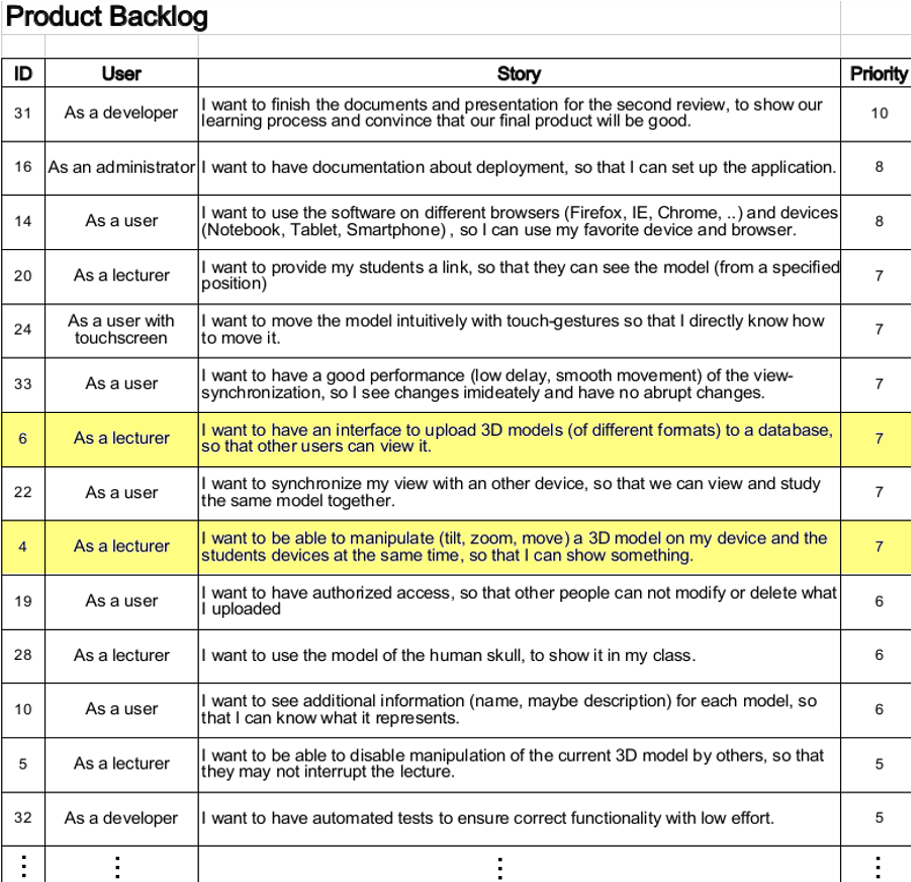
\includegraphics[width=.9\textwidth]{images/product-backlog.png}
    \end{column}
  \end{columns}
\end{frame}

%Transition from what we do to how we do it

\section{Definition of Done}

\begin{frame}
  \frametitle{Definition of Done \textcolor{green!60!black}{(improvements since first review)}}
  \begin{columns}
  \begin{column}{0.5\textwidth}  
  \begin{description}[]
    \item[Short definition of done] \hfill \\
    \item[Git Usage] \hfill \\
    \begin{itemize}
      \item Branching work-flow
      \item Commit Messages
      \item Basic and necessary commands
      \item \textcolor{green!60!black}{Dos and Don'ts}
    \end{itemize}
    \item[Programming Conventions] \hfill \\
    \begin{itemize}
      \item JS, HTML, CSS, \textcolor{green!60!black}{PHP, MySQL}
      \item Mostly Google Guidelines
    \end{itemize}
    \end{description}
  \end{column}
  \begin{column}{0.5\textwidth}  
    \begin{description}[]
    \item[Testing] \hfill \\
    \begin{itemize}
      \item Manual system-tests
      \item \textcolor{green!60!black}{Automated front/back-end tests}
    \end{itemize}
    \item[Gantt Chart] \hfill \\
    \item[Technologies] \hfill \\
    \begin{itemize}
    \item MeshProcessing, RoleSDK, XAMPP, X3DOM, Downsampling, Format conversion
    \end{itemize}
  \end{description}
  \end{column}
  \end{columns}
\end{frame}

\section{Gantt Chart}

\begin{frame}
  \frametitle{Gantt Chart}
  \begin{center}
    \only<1>{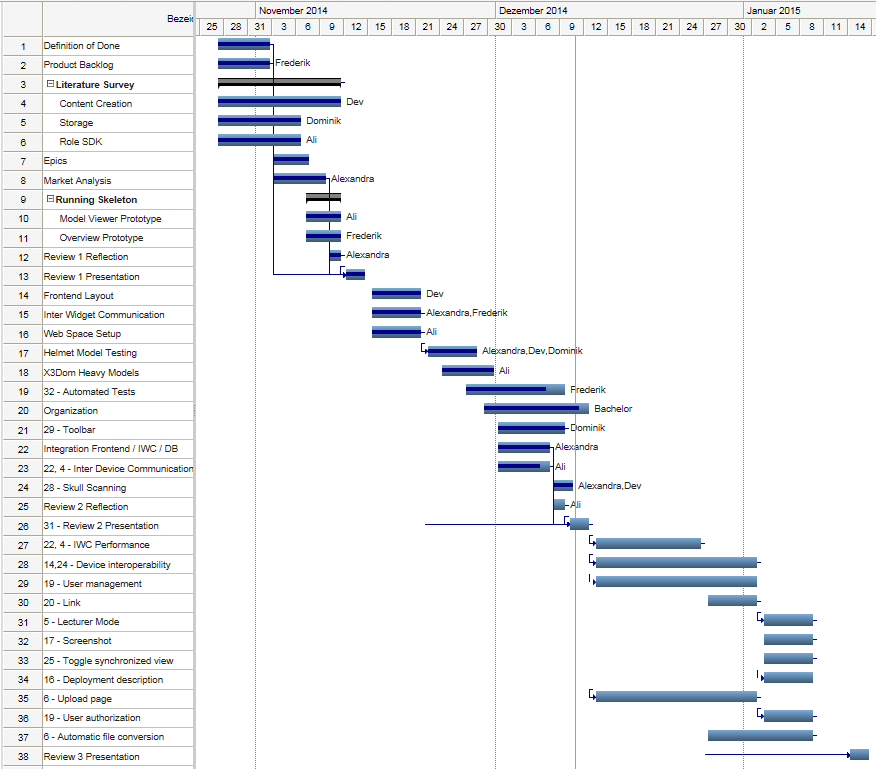
\includegraphics[width=0.8\textwidth]{images/GanttComplete.png}}
    \only<2>{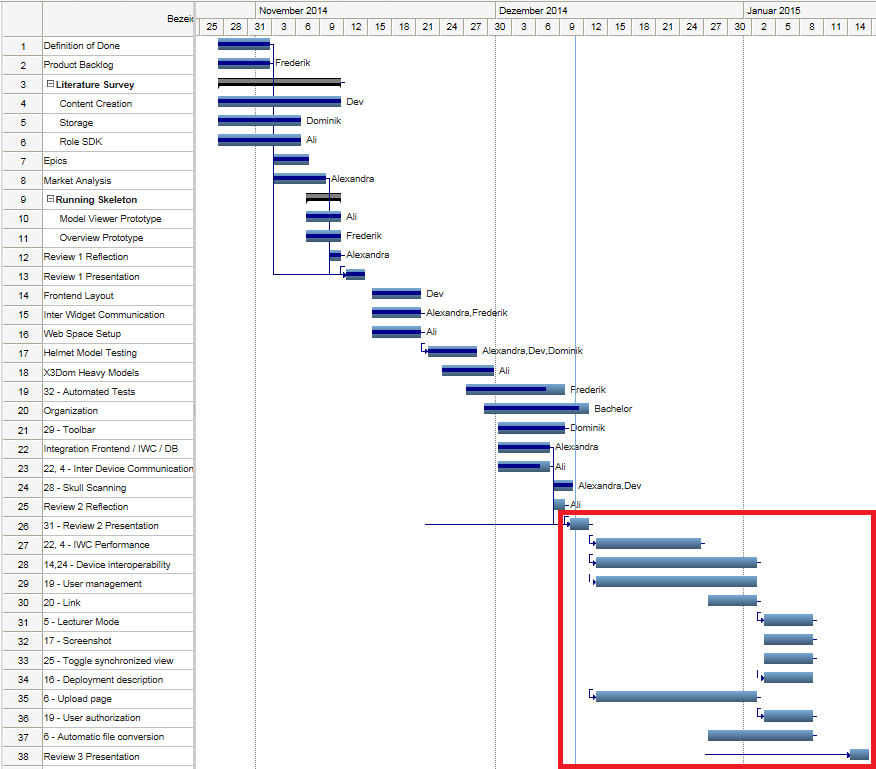
\includegraphics[width=0.8\textwidth]{images/GanttCompleteAnnotated.png}}
    \only<3>{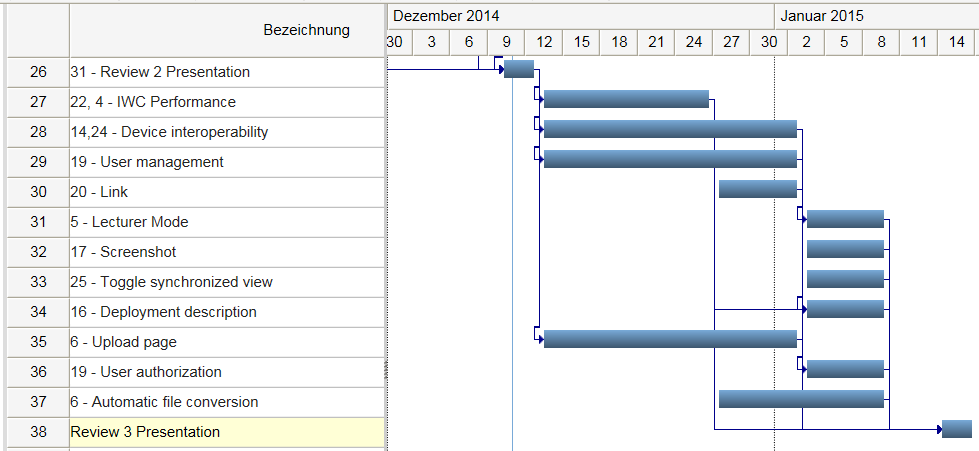
\includegraphics[width=\textwidth]{images/Gantt.png}}
  \end{center}
\end{frame}

\section{Reflection}

\begin{frame}
  \frametitle{Reflections on Team Process}
  \begin{columns}
  	\begin{column}{0.8\textwidth}
   	  \begin{description}[]
        \item[Workflow] \hfill \\
        \begin{itemize}
          \item Team meetings are more often
          \item Live web server, updated every integration
          \item GitLab issue tracker for internal organization and customer contact
        \end{itemize}
  
        \bigskip
        \item[New Colleagues] \hfill \\
        \begin{itemize}
          \item Orientation phase completed
          \item Tasks and responsibilities
          \item Full time support
        \end{itemize}
      \end{description}
    \end{column}
    \begin{column}{0.2\textwidth}
   	  
\includegraphics[width=.9\textwidth]{images/gitlab.png}\\
      \vspace*{2cm}
      
\includegraphics[width=\textwidth]{images/teamwork.jpg}
    \end{column}
  \end{columns}
\end{frame}


\begin{frame}
  \frametitle{Reflections on Team Process}
  \begin{columns}
    \begin{column}{0.7\textwidth}
      \begin{description}[]
        \item[Four Areas of Organizational Performance] \hfill \\
        \begin{itemize}
          \item Decreasing the learning curve of new employees
          \item Responding more rapidly to customer needs and inquiries
          \item Reducing rework and preventing “reinvention of the wheel”
          \item Spawning new ideas for products and services
        \end{itemize}
        \it{Source: IBM Systems Journal, Vol 40, No 4}
      \end{description}
    \end{column}
    \begin{column}{0.3\textwidth}
      
\includegraphics[width=.9\textwidth]{images/ibm.jpg}
    \end{column}
  \end{columns}
\end{frame}

\section{Demo}

\begin{frame}
  \frametitle{Demo}
  
\includegraphics[width=\textwidth]{images/demo}
\end{frame}

\section{Automated Testing}

\begin{frame}
  \frametitle{Automated Testing}
  \begin{columns}
    \begin{column}{0.8\textwidth}
      \begin{description}[]
        \item[Frontend] \hfill \\
        \begin{itemize}
          \item Records user interaction on a website
          \item Executes the recordings automatically
          \item Extend with assertions and verifications
        \end{itemize}

        \bigskip
        \item[Backend] \hfill \\
          \begin{itemize}
            \item JavaScript
            \item Write test suites containing multiple tests (specs)
            \item Execute tests by calling web page
        \end{itemize}
      \end{description}
    \end{column}

    \begin{column}{0.2\textwidth}
      
\includegraphics[width=.9\textwidth]{images/selenium.png}\\
      % Source: http://www.seleniumhq.org/images/big-logo.png
      \vspace*{2cm}
      
\includegraphics[width=\textwidth]{images/jasmine.png}
      % Source: http://jasmine.github.io/images/jasmine-horizontal.svg
    \end{column}
  \end{columns}
\end{frame}

\section{Conclusion}

\begin{frame}
  \frametitle{Conclusion and next steps}
  \begin{description}[]
    \item[Conclusion] \hfill \\
    \begin{block}{}
      \centering{
        \begin{itemize}
          \item Improvements in organization and requirements
          \item Frontend prototype of final product for further evaluation
          \item Basic functionality working (device communication)
          \item Automated tests to ensure quality
        \end{itemize}
      }
    \end{block}
    \item[Next Steps] \hfill \\
      \begin{itemize}
        \item Improving performance
        \item Testing device interoperability
        \item User management
        \item Upload page
      \end{itemize}
  \end{description} 
\end{frame}

\end{document}
